\begin{figure*}
  \centering
  \begin{subfigure}[b]{\textwidth}
    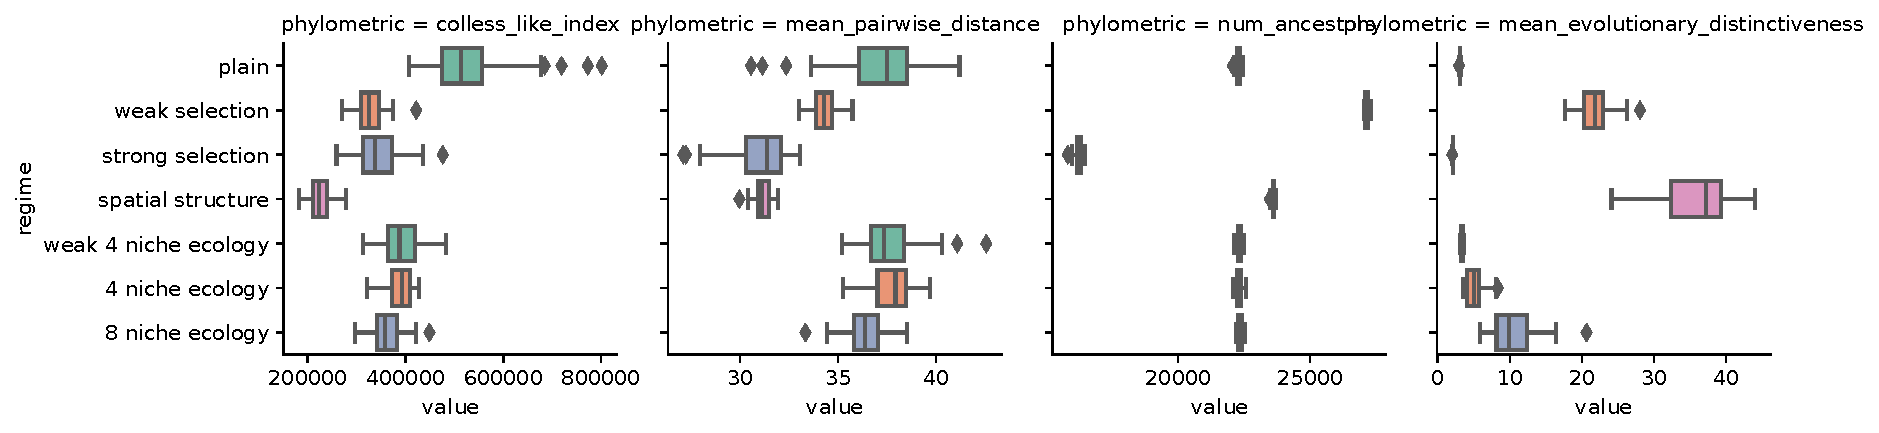
\includegraphics[width=\textwidth]{binder/binder/teeplots/col=phylometric+epoch=7+mut_distn=np.random.standard_normal+viz=boxplot+x=value+y=regime+ext=.pdf}
  \caption{%
    Distribution of tree phylometrics measured with perfect phylogenetic tracking across surveyed evolutionary regimes.
    Sample sizes of $n=50$ replicates define each depicted distribution.
  }
  \label{fig:perfect-tree-phylometrics}
  \end{subfigure}
  \vspace{1cm}
  \begin{subfigure}[b]{\textwidth}
  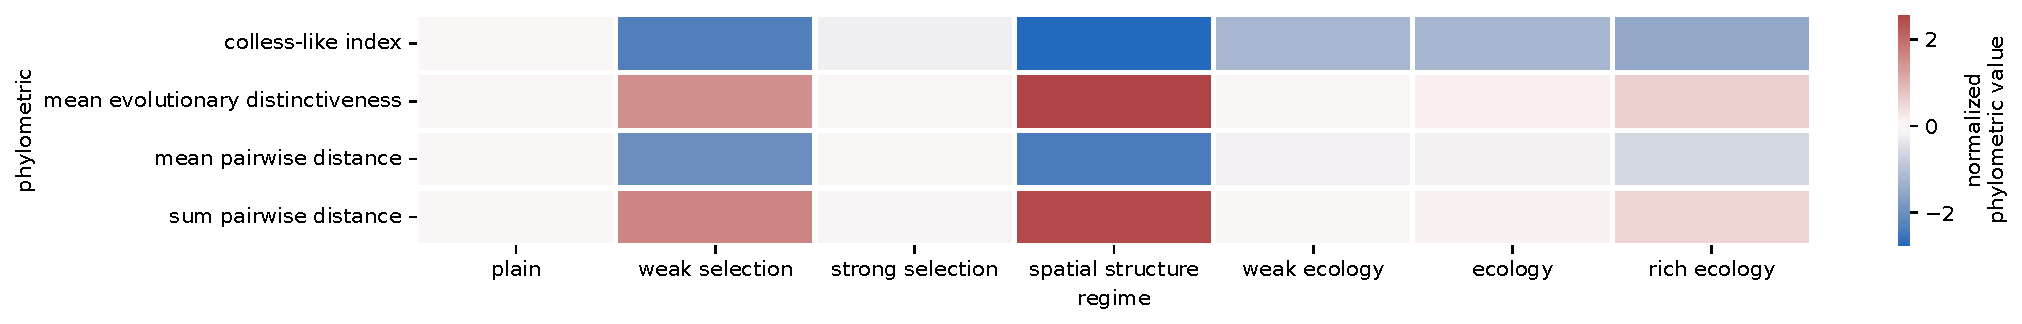
\includegraphics[width=\textwidth]{binder/binder/teeplots/epoch=7+mut_distn=np.random.standard_normal+normed=true+viz=heatmap+x=regime+y=phylometric+ext=.pdf}
  \caption{%
    Heatmap of normalized tree phylometrics across surveyed evolutionary regimes, calculated on perfect-fidelity simulation phylogenetic records.
    See Supplementary Figure \ref{fig:perfect-tree-phylometrics-heatmap-sensitivity-analysis} for results under sensitivity analysis conditions.
  }
  \label{fig:perfect-tree-phylometrics-heatmap}
  \end{subfigure}
  \vspace{1cm}
  \begin{subfigure}[b]{\textwidth}
    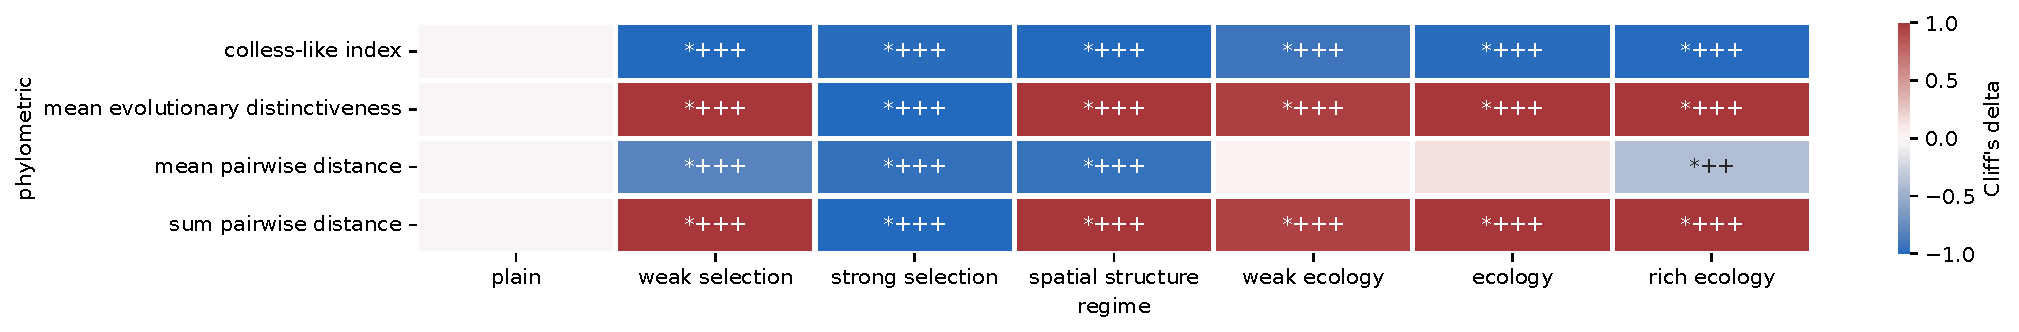
\includegraphics[width=\textwidth]{binder/binder/teeplots/epoch=7+mut_distn=np.random.standard_normal+viz=heatmap+x=regime+y=phylometric+ext=.pdf}
    \caption{TODO.}
  \end{subfigure}%
  \begin{subfigure}[b]{\textwidth}
    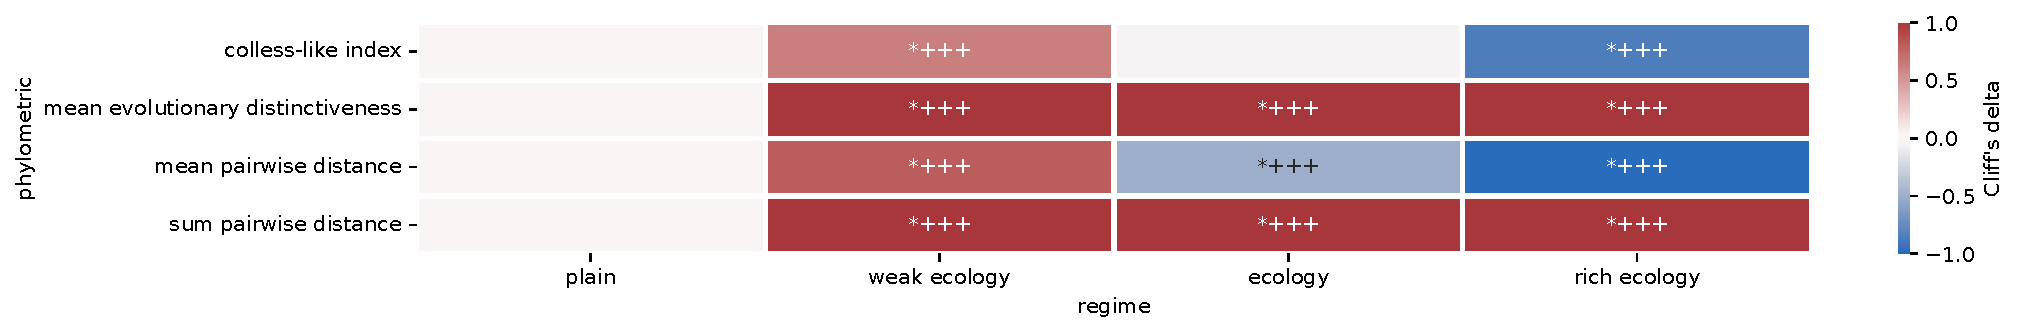
\includegraphics[width=\textwidth]{binder/binder/teeplots/epoch=7+mut_distn=np.random.standard_normal+spatial=true+viz=heatmap+x=regime+y=phylometric+ext=.pdf}
    \caption{TODO}
  \end{subfigure}
  \caption{Heatmap of normalized tree phylometrics across surveyed evolutionary regimes, calculated on perfect-fidelity simulation phylogenetic records.}
  \label{fig:perfect-tree-phylometrics-compound}
\end{figure*}
